\documentclass[11pt]{article}
\usepackage[a4paper,margin=2.5cm]{geometry}
\usepackage[utf8]{inputenc}
\usepackage[T1]{fontenc}
\usepackage{graphicx}
\usepackage{booktabs}
\usepackage{amsmath}
\usepackage{authblk}
\usepackage[numbers,sort&compress]{natbib}
\usepackage[hidelinks]{hyperref}
\usepackage{setspace}
\usepackage{lineno}
\onehalfspacing
\linenumbers
\graphicspath{{figures/}}

\title{\textbf{Mapping intra-urban social deprivation from Sentinel imagery using
only municipal aggregate labels}}
\author[1]{Dagoberto Pulido Arias}
\affil[1]{Independent researcher, Mexico. Correspondence: dagopa.1010@gmail.com}
\date{}

\begin{document}
\maketitle

\begin{abstract}
\noindent Most countries publish social statistics as administrative aggregates;
almost none publish them at neighborhood level. We measure how much neighborhood
detail aggregates and free satellite imagery jointly recover. Trained only on five-level
deprivation aggregates of Mexican municipalities, with no spatial annotation, and
scored against fully held-out census-tract grades, the map reaches a
within-municipality rank correlation of $\rho = 0.20$ on fourteen held-out test
cities with a DOFA base backbone and $0.23$ with DOFA large: 84\% and 77\% of what
the same features attain there under full tract supervision ($0.23$ and $0.30$; 90\%
and 76\% on the validation cities used for model selection). More aggregates
keep buying map, state aggregates forfeit part of it, one national figure erases it, and
optical content matters where resolution does not. The maps close 31--66\% of the
aggregate-to-census targeting gap on test, replicate against an independent
institution's index, beat the incumbent wealth index where selection occurred and match
it on test, and order Bogot\'a's block strata without retraining. Repeating the design
abroad on each country's own municipal aggregates, Colombia's poverty rate and Brazil's
mean income, recovers a within-municipality ordering of block strata in Bogot\'a
($\rho = 0.21$) and of tract income across 47 Brazilian municipalities ($0.12$) from 35
and 48 bags, the small-supply end of the Mexican curve. Against free global grids the
margin is resolvable only for population; nighttime lights order tracts inside a
municipality as well as the maps do, and feeding those grids to the model as inputs lifts
the fully supervised bound by $0.03$ without lifting the weakly supervised map. Attention-based multiple-instance learning fails here
for a measurable, structural reason, and ensembling over seeds yields no usable
uncertainty layer: an honest 90\% grade interval spans 1.7 to 1.9 of the five levels.
Every result is reported for both backbones; under grouped cross-validation over all
138 cities the larger one improves the map by $0.03$ [$0.01$, $0.05$].
\end{abstract}

\begin{center}
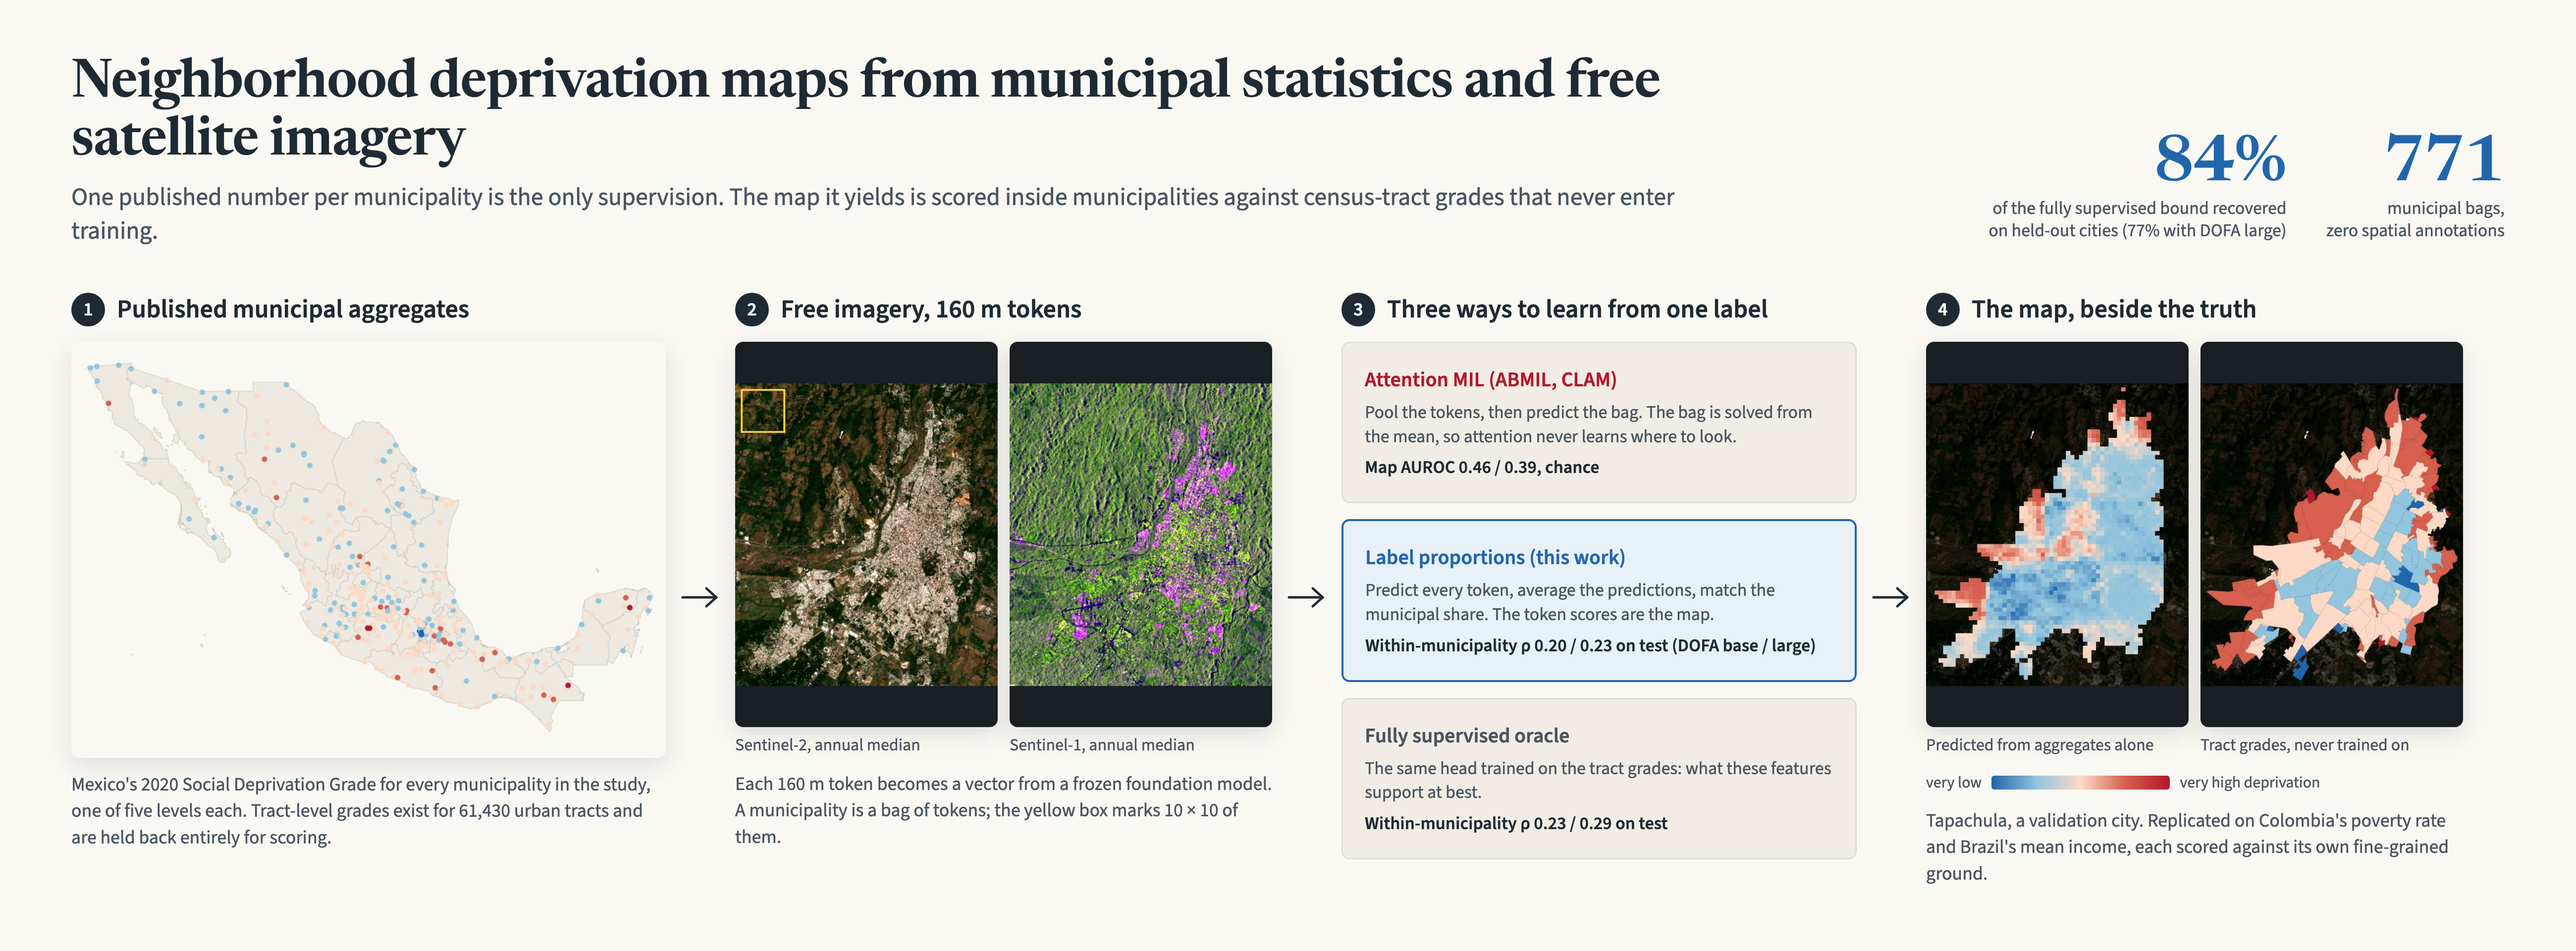
\includegraphics[width=\linewidth]{graphical_abstract.png}\\[2pt]
{\small\textbf{Graphical abstract.} What the model is told, what it sees, the three
ways of learning from one label per municipality, and the map beside the tract truth it
is scored against; every panel is a project artifact.}
\end{center}

\section{Introduction}

Census-quality social data is expensive, and most of the world sees it roughly once a
decade. In between, and below the level the tables are published at, policy relies on
aggregates: municipal indices and district averages. Predicting an aggregate somewhere
else and disaggregating it in place are different tasks, and the second is the one
targeting decisions require: a mayor already knows the municipality is poor but lacks a
map of which neighborhoods are poorest.

A decade of work has established that satellite imagery and machine learning predict
socioeconomic indicators across space. Jean et al.~\cite{jean2016} transferred features
learned from nighttime lights to daytime imagery and explained a large share of the
variation in survey-measured consumption across African clusters; Yeh et
al.~\cite{yeh2020} extended the approach to seventeen years and twenty-three countries;
Head et al.~\cite{head2017} showed that the transfer degrades away from the settings it
was fit in; Engstrom et al.~\cite{engstrom2022} and Ayush et al.~\cite{ayush2021} reached
finer targets with sub-metre imagery; Rolf et al.~\cite{rolf2021} showed that random
convolutional features suffice for many such tasks; Chi et al.~\cite{chi2022} released a
global 2.4 km wealth grid, and Lee and Braithwaite~\cite{lee2022} district-level poverty
maps for sub-Saharan Africa. Burke et al.~\cite{burke2021} review the field. The design
these studies share is that labels come from household surveys at the cluster or
district where they were collected, models are scored on held-out clusters or districts,
and the products steer program targeting at that resolution~\cite{aiken2022}. Ordering
neighborhoods inside a city is rarely the target and, because independent ground at
that resolution is rare, rarely evaluated.

Two literatures do address the intra-urban scale, from opposite directions. Slum mapping
from imagery has fifteen years of results~\cite{kuffer2016}, almost all of them
supervised by digitized settlement delineations, that is, by the fine labels a
statistics office lacks. Dasymetric and disaggregation methods distribute a known
aggregate over covariates~\cite{stevens2015,wardrop2018}, but they are validated where
the aggregate is known and rarely against an independent fine-grained truth. Both
inherit the caveats of any spatially aggregated label, the modifiable areal unit
problem~\cite{openshaw1984} and the ecological fallacy, which we quantify rather than
assume away.

The learning problem in between, one label per administrative unit and a map wanted
inside it, is weak supervision. Multiple-instance learning treats the unit as a bag of
image tokens and the aggregate as its label~\cite{carbonneau2018}; attention-based
pooling~\cite{ilse2018}, refined for computational pathology~\cite{lu2021}, is its
standard localizer and the natural first candidate here. Learning from label
proportions~\cite{quadrianto2009,yu2013,ardehaly2017,dulac2019} is the sibling
formulation in which the bag label is the share of positive instances, which is
literally what a municipal deprivation figure is. Weakly supervised segmentation of
satellite imagery has used image-level tags~\cite{wang2020}, and the arrival of
self-supervised Earth-observation foundation models~\cite{cong2022,wang2023,xiong2024}
means the representation can be held fixed and the question reduced to what the weak
labels can teach a small head on top of it.

We ask the disaggregation question quantitatively: how much neighborhood detail can be
recovered from a country's published aggregates combined with free imagery? We frame the
answer as an exchange rate between the number and granularity of published aggregates
and the within-municipality detail they recover, and we measure it in a country that
publishes ground truth at both levels. Mexico publishes its Social Deprivation Grade
(GRS) both as municipal aggregates and for 61{,}430 urban census tracts
(AGEB)~\cite{coneval2020}; we train only on the former and score maps against the
latter, held out entirely, in cities the model never saw (Fig.~\ref{fig:design}).

\begin{figure}[htbp]
\centering
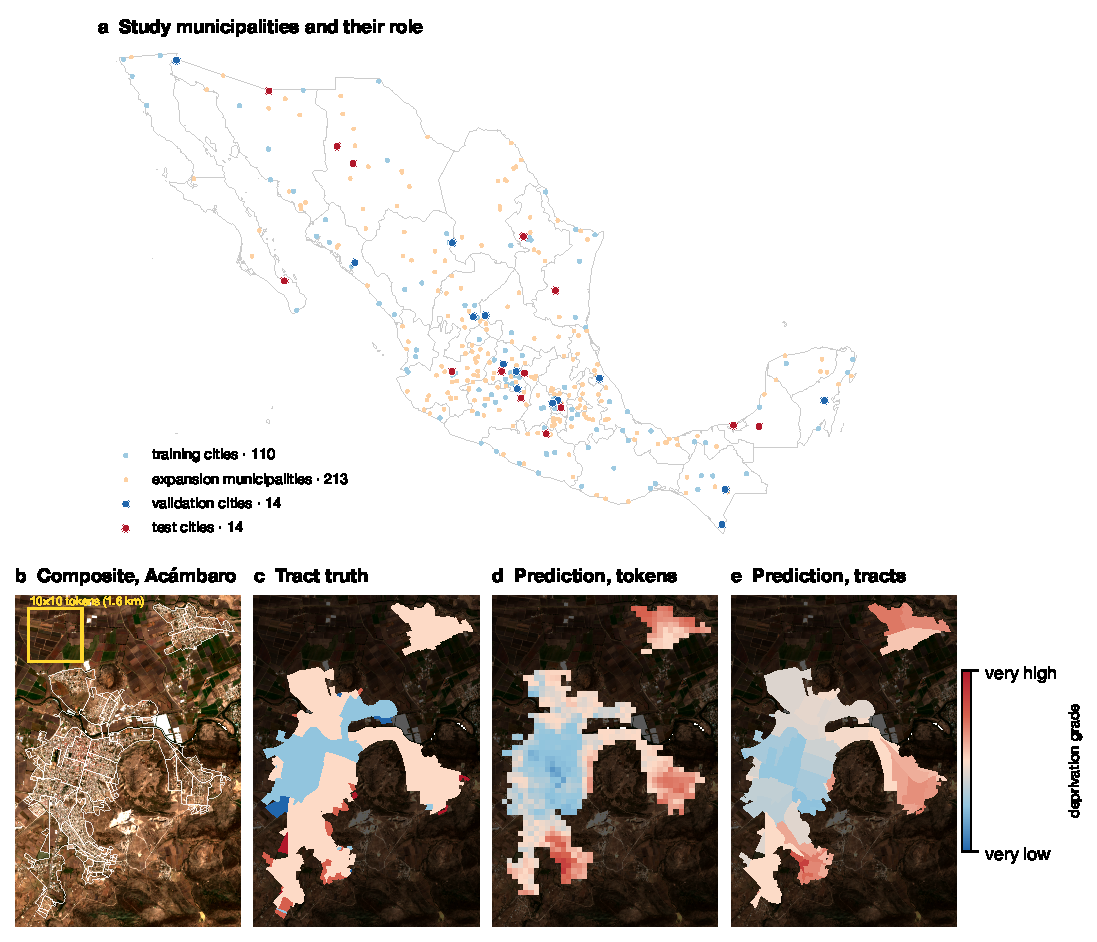
\includegraphics[width=\linewidth]{fig1_design.pdf}
\caption{\textbf{Study design.}
\textbf{a}, The 351 study units: 110 training cities, the 213-municipality expansion
toward the deprived half of urban Mexico (municipalities overlapping held-out ground
excluded), 14 validation and 14 held-out test cities. A city box is a conurbation and
typically yields several municipal bags, which is how 351 units produce 771 bags. \textbf{b}, What the
model consumes: the 2020 Sentinel-2 median composite of Ac\'ambaro (a validation city)
with AGEB boundaries overlaid; tokens of 160 m tile the box. \textbf{c}, The tract
truth, which never enters training, each AGEB polygon filled with its GRS grade. \textbf{d}, What the model
produces: the token-level deprivation score from municipal aggregates alone (DOFA base
backbone), on the same scale. \textbf{e}, The same prediction averaged to the tract, the unit at which every
evaluation in this paper scores it. Ac\'ambaro is the validation municipality with the
highest within-municipality agreement among those holding all five grades ($\rho =
0.51$ at token level); the validation median over municipalities is $0.27$, so the panel
shows the map where it works, with the typical case stated here.}
\label{fig:design}
\end{figure}

Three design choices constrain the measurement. Supervision is weak: a model sees a bag
of image tokens for a municipality and one vector, the population shares at each grade
threshold, with no spatial annotation of any kind. Every comparison is scored
\emph{within} municipalities, because ordering tracts across cities is mostly solved by
knowing which city is poor (pooled correlations run near 0.46 against 0.23 within, at
the same operating point). And an oracle trained directly on the held-out tract labels
bounds what the frozen representation supports, so weak supervision is always reported
as a fraction of a measured upper bound.

The contributions are the following. (1) A measured exchange rate: on fourteen held-out
test cities, the national supply of municipal aggregates recovers 84\% of the fully
supervised bound within municipalities with a DOFA base backbone and 77\% with DOFA
large, whose maps are higher in absolute terms, and the curve along the number of
aggregates, their granularity and the sensor content is reported on both splits and both
backbones, which are compared by grouped cross-validation over all 138 cities. (2) A structural
failure of attention-based multiple-instance learning in this setting, with its cause,
and the observation that the only selection signal weak supervision may use, bag error,
is close to uninformative about map quality. (3) Four external checks of the map, against
Meta's wealth index, an independent institution's index, simulated targeting, and free
global grids as competitors and as inputs. (4) A replication of the design on Colombia's
and Brazil's own municipal aggregates, scored against their own fine ground. (5) A frozen
benchmark with held-out instance labels, released so that weakly supervised mapping can
be evaluated on the quantity it claims.

\section{Study area and data}

The study covers urban Mexico: the 138 cities of the national set, stratified by size and
deprivation, plus 213 municipalities added to reach the deprived half of the urban
population that large-city samples miss, 424 boxes in all; a city box is a conurbation
and typically spans several municipalities. Imagery is the Sentinel-2 L2A and Sentinel-1
RTC annual median composites for 2020 on a 10 m grid, read by window from the
cloud-optimized GeoTIFFs of Microsoft Planetary Computer. Labels are the CONEVAL GRS
2020~\cite{coneval2020}: municipal-level population shares at each of four grade
thresholds supervise training, and AGEB-level grades are used only for evaluation and
for the oracle. Auxiliary evaluation sources are CONAPO's urban marginalization index
2020~\cite{conapo2020}, ESA WorldCover 2020~\cite{worldcover}, Meta's Relative Wealth
Index~\cite{chi2022}, the GHSL R2023A grids~\cite{ghsl2023}, harmonized nighttime
lights~\cite{li2020}, IBGE's AGSN 2019~\cite{ibge2019} and Bogot\'a's district
stratification~\cite{bogota}. For training abroad: Colombia's municipal
multidimensional poverty rate (DANE, census 2018)~\cite{dane_ipm} with the MGN 2023
municipal boundaries~\cite{mgn2023}, and Brazil's municipal mean and tract median
monthly income of the household head (IBGE, census 2022)~\cite{ibge2022} with the 2022
census tract geometries.

\section{Methods}

\subsection{Bags, labels and features}

A bag is a municipality (771 after exclusions) and its instances are 16-pixel tokens
(160 m) encoded by a frozen DOFA foundation model~\cite{xiong2024}, both sensors fused
per token. Municipalities contributing ground to any held-out city are excluded from
the expansion; an earlier version leaked nine validation municipalities this way,
detectable only at bag level, and every affected number was re-measured. A two-layer
head on standardized frozen features predicts four cumulative-grade probabilities per
token; the bag prediction is the mean of the token predictions, fit with binary
cross-entropy against the municipal population shares; each token's hidden
representation is concatenated with the mean of its 8 grid neighbors (480 m),
computed city-wide at inference. Fourteen configurations varied one ingredient each
(learning rate 5e-5 to 1e-3, hidden width 64 to 512, dropout 0 to 0.5, weight decay,
loss, input standardization), then a combination round; standardized inputs with binary
cross-entropy won on bag error over five grouped training folds. The oracle is the same
head trained on tract labels with the same context, and bounds what the representation
supports ($\rho = 0.251$ with context and $0.202$ without for DOFA base; $0.318$ and
$0.260$ for DOFA large). The two other axes of the
curve reuse the pool unchanged: granularity relabels every bag with its state's or the
national aggregate, and content re-encodes the optical composite block-averaged to the
radar's 20 m effective resolution, or uses each sensor alone.

\paragraph{Two backbones} Every experiment in this paper is run on two frozen backbones
of the same family, DOFA base (768 dimensions per sensor, 1536 fused) and DOFA large
(1024 per sensor, 2048 fused), with the same head, protocol, seeds and splits; every
table reports both and every figure draws DOFA large hatched or with hollow markers. The
head was tuned on DOFA base and reused unchanged on DOFA large. Fourteen cities are too
few to separate backbones, so they are compared by grouped cross-validation over all
138 cities of the partition. The cities are dealt into five folds stratified as the
partition was, by size and by share of high-deprivation tracts; for each fold the head
trains on the remaining cities plus the expansion municipalities, with every bag sharing
a municipality key with the held-out fold removed, and early stopping uses bag-level
error on 14 cities drawn from the training side, so the held-out fold plays no part in
selection. Three seeds per fold; the seed-mean token scores of every held-out city are
pooled and scored with the same metrics as the rest of the paper, with 95\% percentile
bootstrap intervals that resample cities, and the difference between two backbones is
bootstrapped on the same city draws. Copernicus-FM base~\cite{wang2025cfm}, which
additionally takes the location, date and footprint of each window, was compared the
same way and appears in that comparison only.

\subsection{Partition, selection and statistics}

The 138 cities are dealt 110/14/14 into training, validation and test, stratified by
size and deprivation, with no city split across sets. Hyperparameters are selected on
grouped training folds under bag error; early stopping and the choice among reported
configurations use the validation cities; the test cities are held out for reporting.
Comparisons are paired by municipality over three seeds (0, 1 and 2 throughout); every
interval on a within-municipality mean is a city-clustered bootstrap (2{,}000
resamples), and curve error bars are s.d. over seeds. The code is Python 3.12 with
PyTorch, rasterio, geopandas and scikit-learn, pinned by the repository's
\texttt{uv.lock}; all experiments ran on one Apple-silicon laptop (MPS backend). The
seven municipalities excluded from the expansion for insufficient composite depth or
persistent acquisition errors (Table~\ref{tab:exclusions}) are the only data exclusions. The
full pipeline, frozen vectors, labels, splits and protocol are released, and every
figure regenerates from one canonical results file.

\begin{table}[htbp]
\centering
\caption{Municipalities excluded from the expansion for insufficient optical depth or
persistent acquisition errors; the guard requires eight observations per pixel and
excludes shallow ground instead of compositing it.}
\begin{tabular}{ll}
\toprule
Municipality & Reason\\
\midrule
Amozoc; Comalcalco; Hidalgo del Parral; & composite below the eight-observation\\
Lagos de Moreno; Nuevo Casas Grandes & depth floor (optical arm)\\
La Independencia & inconsistent tract geometry\\
El Marqu\'es & repeated acquisition timeouts\\
\bottomrule
\end{tabular}
\label{tab:exclusions}
\end{table}

\subsection{External checks}

Five checks measure the map against ground that never entered training. \emph{RWI
pairing}: each AGEB takes the RWI value of the nearest grid point to its centroid; the
model is averaged token-to-tract; both are scored on the 2{,}958 shared AGEB in the 22
municipalities with at least 20 scored tracts and more than one grade, and the interval
is a city-clustered bootstrap of the per-municipality difference. \emph{Global
products}: four free layers stand in for what a practitioner would download instead of
training anything, GHSL built-up surface (R2023A, 2020 epoch, 100 m), GHSL average net
building height (R2023A, 2018, the only epoch published), GHSL residential population
(R2023A, 2020)~\cite{ghsl2023}, and the harmonized global nighttime lights of 2020,
VIIRS-derived and expressed on the DMSP digital-number scale at 30
arcsec~\cite{li2020}. Nighttime lights come from the harmonized series because the EOG
annual composite requires an account; the harmonized layer is the same VIIRS
observation on a coarser grid and a compressed scale, which is a handicap for
intra-urban ranking and is reported as such. Each product is averaged over the pixels
whose centers fall inside a tract, in the product's own grid so nothing resamples it; a
tract smaller than one cell takes the value at a representative interior point, and the
count of such fallbacks is reported. All four are used in practice as development
proxies, so deprivation is taken as the negative of each, an orientation fixed before
any correlation was computed; scoring is the RWI protocol unchanged.
\emph{Targeting simulation}: for each validation city and budget $q \in \{5, 10, 20,
30\}\%$ of population, tracts are funded in the order given by each allocator (municipal
aggregate with ties broken at random over 200 draws, the map's tract-mean score, or
tract truth), with the marginal tract funded fractionally, so the truth ordering
upper-bounds both by construction; the outcome is the population living in high or
very-high grade tracts among those reached, pooled over cities before the gap ratio is
formed. \emph{Areal units}: tracts are binned by tokens contained (1--3, 4--9, 10--19,
20--49, $\geq$50); within-municipality correlations use municipalities with at least
ten tracts in the bin. \emph{Border test}: adjacent token pairs (160 m apart) are
classed by what their midpoint crosses; the excess mean absolute score jump of
same-grade municipal-border pairs over same-tract pairs is city-bootstrapped, and
same-grade AGEB-border pairs inside one municipality are the placebo.

\subsection{Uncertainty and intervals}

Uncertainty is read from the three training seeds: a tract's map value is the mean of
its per-seed tract means and its spread is their standard deviation, a quantity
computable with no labels. Three things are then asked of that spread. Whether it ranks
the errors, as the within-municipality correlation between spread and the absolute
distance from an isotonic score-to-grade map fitted on validation. Whether discarding
the least confident tracts inside each municipality raises the correlation over what
remains; the panel of municipalities is fixed to those that stay above twenty tracts at
every point of the sweep, so the curve cannot rise by attrition. And whether an interval
can be attached, by split conformal calibrated on the validation cities and evaluated on
the test cities, with the absolute isotonic residual as the nonconformity score. Two
rules are compared: the marginal quantile, which treats all tracts as exchangeable, and
a clustered rule that takes each calibration city's quantile and then the 90th
percentile across cities. Per-city coverage is reported for both.

\subsection{Global products as input features}

The same four products, plus the eleven WorldCover class fractions and the NDVI mean and
dispersion of the composite, are also tested as inputs. Each is reprojected onto the 10 m
grid and averaged inside every 160 m token (population and built surface as
$\log(1 + x)$), giving four GHSL and light columns and thirteen WorldCover columns
appended to the 1{,}536 encoder dimensions. Two fusions are compared on the full pool,
three seeds each, against the canonical head: early, the columns enter the projection
with the encoder vector; late, they bypass it and enter the scoring layer beside the
hidden representation, each with a weight of its own per threshold. The oracle is
re-measured with the same inputs, standardized, since a nighttime-light column near 45
on an unstandardized scale would dominate the first layer; its no-extras reference is
re-run under the same standardization, and differences are paired by municipality with
a city-clustered bootstrap.

\subsection{Transfer to Colombia and Brazil}

Zero-shot: Bogot\'a and Rio get the same 2020 composite protocol; tokens are scored by
the three final seeds with Mexican standardization statistics, deliberately unadapted.
Rio's evaluation is restricted to tokens with WorldCover built fraction $\geq 0.10$.

Training on local aggregates: six composited boxes (Bogot\'a, the Aburr\'a valley,
Cali; Rio, S\~ao Paulo, Belo Horizonte) are cut into 160 m tokens, encoded by the same
frozen model, and kept where the WorldCover built fraction is $\geq 0.10$. A bag is a
municipality with at least 5\% of its area inside a box and at least 32 built tokens,
assigned from each country's official boundaries: 35 bags in Colombia, 48 in Brazil.
The label is what each office publishes at municipal level and nothing finer: Colombia's
multidimensional poverty rate, a share that enters the one-output label-proportion head
unchanged; Brazil's mean monthly income of the household head, mapped to a deprivation
share by scaling minus its logarithm to $[0, 1]$ over the country's bags, a monotone
transform carrying no spatial information. The head, context and training settings are
the Mexican ones with a single threshold, 40 epochs, no early stopping. Evaluation runs
under five grouped folds by municipality and three seeds, so every token is scored by a
model that never saw its municipality's label, against fine ground that never enters
training: Bogot\'a's block strata (nearest block within 120 m, inverted; 12{,}738
tokens) and, in Brazil, minus the log median income of the household head in the census
tract containing the token (110{,}728 tokens across 47 municipalities with at least 20
such tokens). Two further rows share the folds: the Mexican heads fine-tuned on the local
aggregates (projection and scaler loaded, scoring row initialized as the mean of the four
Mexican thresholds, learning rate $5 \times 10^{-5}$), and the oracle, the same head
trained on the token truth. Colombia's truth exists in Bogot\'a alone, so its oracle folds
over 3.2 km spatial cells inside the city; Brazil's oracle keeps the municipal folds.

\section{Results}

\subsection{Supervision efficiency}

Figure~\ref{fig:curve} shows the measurement on a pool of 771 municipal bags: the 110
training cities plus 213 municipalities added expressly to cover the deprived half of
urban Mexico that large-city samples miss (Fig.~\ref{fig:design}a; municipalities
overlapping any held-out city's ground are excluded, Methods). Every row below
reports the fourteen held-out test cities with validation-selected models, for DOFA base
and DOFA large in that order; validation values are shown beside them as the selection
benchmark. \textbf{Quantity} (Fig.~\ref{fig:curve}a): fifty aggregates yield
$\rho = 0.15$ and $0.18$ within municipalities on validation; the full national supply
yields $0.196$ and $0.226$ on test against fully supervised upper bounds of $0.233$ and
$0.295$ there (per-point values in Table~\ref{tab:curve}), a recovery of 84\% and 77\%
(validation: $0.227$ of $0.251$ and $0.242$ of $0.318$, 90\% and 76\%). Pairing model
and oracle by municipality, the city-clustered bootstrap puts the test fraction of DOFA
base at $0.85$ with a wide interval [$0.29$, $1.83$]; fourteen cities bound the precision,
and it is the point estimate, consistent across splits and backbones, that the title
claims. The larger backbone raises the upper bound by $0.06$ and the map by $0.02$ to
$0.03$ on both splits, so the aggregates recover a smaller share of a richer
representation. The test curve of DOFA base reproduces the rise through 400 aggregates
almost exactly and flattens at the top; DOFA large is higher at every point of the curve
on both splits, most at 100 to 200 aggregates on validation ($0.141 \to 0.199$ and
$0.151 \to 0.231$), where the base representation has not yet begun to rise.
\textbf{Granularity} (Fig.~\ref{fig:curve}b): relabeling the same bags with state-level
aggregates cuts the map from $0.225$ to $\rho = 0.152$ on validation and from $0.195$ to
$0.168$ on test with DOFA base, and from $0.238$ to $0.134$ and from $0.223$ to $0.182$
with DOFA large; a single national aggregate erases it ($0.009$ and $0.010$ validation,
$0.004$ and $-0.002$ test). Recovered map quality falls monotonically with coarser
publication on both splits and both backbones, and with state aggregates the larger
backbone has no advantage. \textbf{Content} (Fig.~\ref{fig:curve}c): block-averaging
the optical input to the radar's 20 m effective resolution costs little on validation
($0.183 \to 0.172$ base, $0.235 \to 0.217$ large) and more on test ($0.179 \to 0.129$
and $0.207 \to 0.191$), while radar sits far below both ($0.006$ and $0.022$ validation,
$0.084$ and $0.016$ test), despite having been the best single sensor at detecting
high-deprivation tracts in our feature-based phase-one baseline (per-city AUROC 0.773
against 0.747 optical). With DOFA large the optical sensor alone reaches what the fused
DOFA base model reaches. Sensor content dominates ground sampling distance, with
resolution carrying a real secondary cost on test; a sensor's prediction accuracy is a
poor guide to its map quality.

\begin{figure}[htbp]
\centering
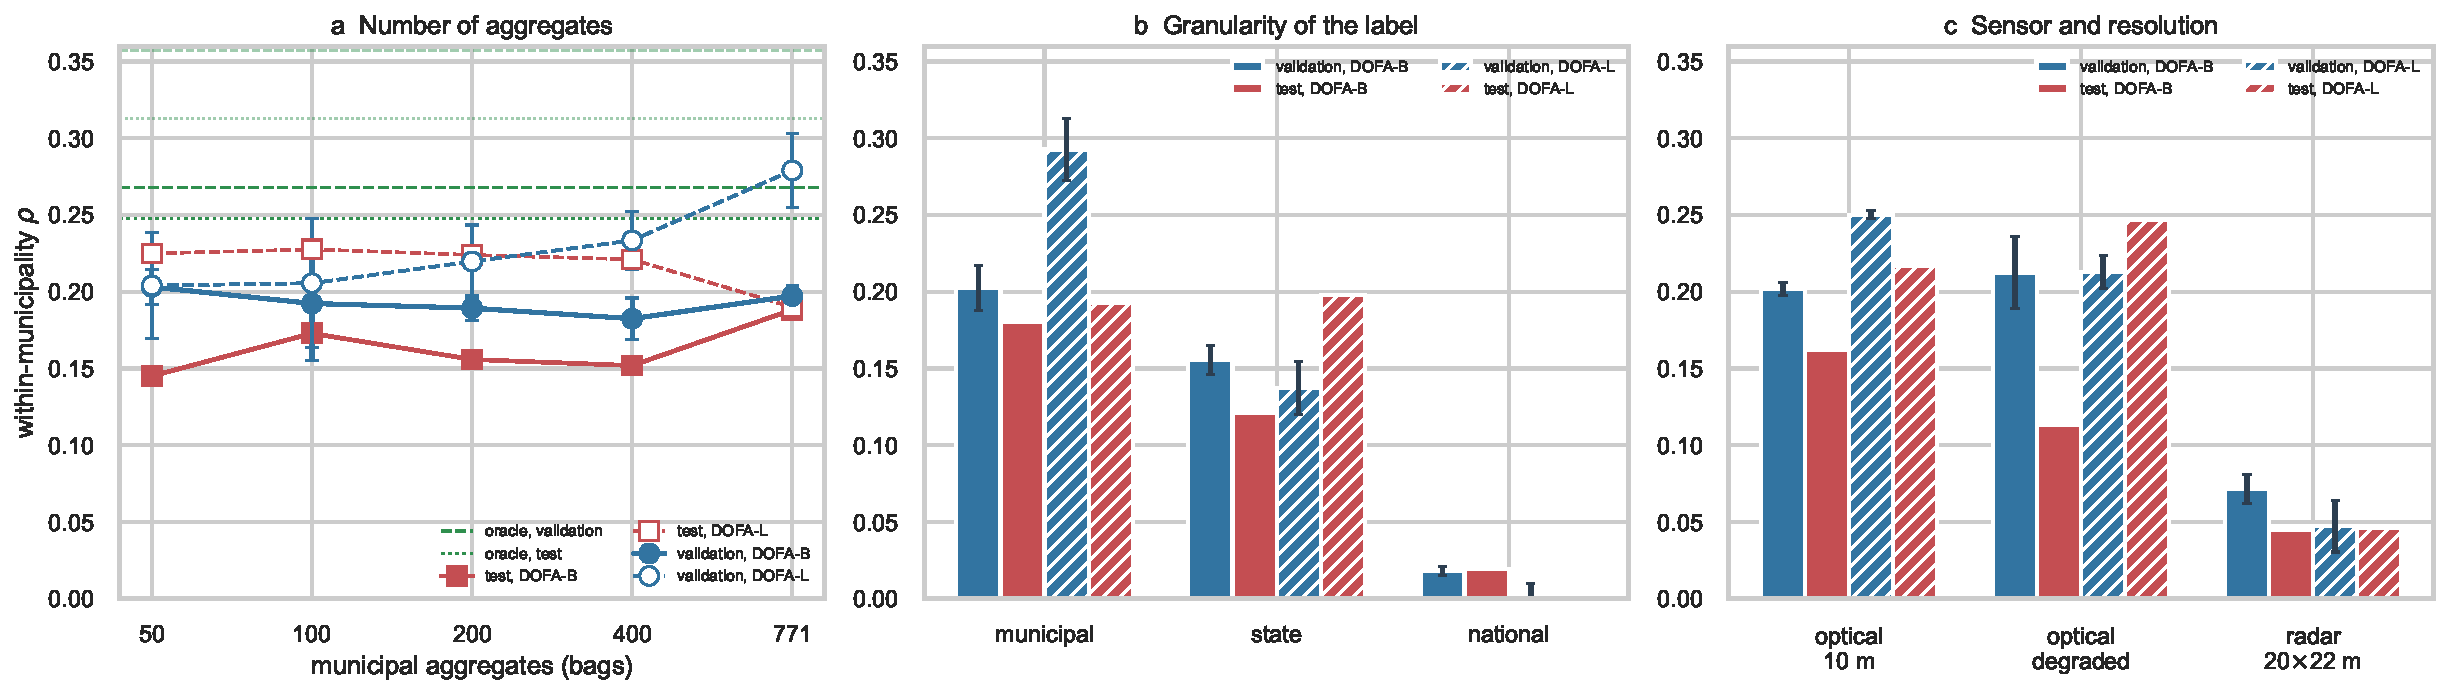
\includegraphics[width=\linewidth]{fig2_curve.pdf}
\caption{\textbf{What the map recovers as a function of the aggregates.} All panels:
mean over three seeds against held-out tract grades, for DOFA base (solid, filled) and
DOFA large (dashed or hatched, hollow); blue, the 14 validation cities used for
selection (error bars, s.d. over seeds); red, the 14 held-out test cities, drawn without
a spread; dashed and dotted green lines, the fully supervised oracle upper bound on each
split ($\rho = 0.251$ validation and $0.233$ test for DOFA base; $0.318$ and $0.295$
for DOFA large, lighter). \textbf{a}, Agreement as a function of how many municipal
aggregates supervise training (nested, grade-stratified sampling). \textbf{b}, The same
771 bags relabeled with coarser aggregates. \textbf{c}, Single-sensor configurations:
degrading optical resolution to the radar's 20 m grain costs little on validation and a
real but secondary amount on test; radar sits far below both with either backbone.}
\label{fig:curve}
\end{figure}

\begin{table}[htbp]
\centering
\caption{The supervision-efficiency curve (Fig.~\ref{fig:curve}a) for both backbones.
Within-municipality Spearman $\rho$ against held-out tract grades, mean over three seeds
(s.d. over seeds on validation); validation cities were used for model selection, test
cities are held out. The last row gives the test value of the retrained models and, after
the semicolon, of the validation-selected saved weights that every downstream analysis
scores.}
\begin{tabular}{rcccc}
\toprule
 & \multicolumn{2}{c}{DOFA base} & \multicolumn{2}{c}{DOFA large}\\
\cmidrule(lr){2-3}\cmidrule(lr){4-5}
Bags & Validation (s.d.) & Test & Validation (s.d.) & Test\\
\midrule
50 & 0.150 (0.006) & 0.156 & 0.183 (0.040) & 0.180\\
100 & 0.141 (0.006) & 0.158 & 0.199 (0.051) & 0.200\\
200 & 0.151 (0.006) & 0.161 & 0.231 (0.023) & 0.172\\
400 & 0.182 (0.017) & 0.192 & 0.222 (0.024) & 0.205\\
771 & 0.227 (0.014) & 0.185; 0.196 & 0.242 (0.006) & 0.219; 0.226\\
\bottomrule
\end{tabular}
\label{tab:curve}
\end{table}

\textbf{Backbone} (Table~\ref{tab:backbone}). Under grouped cross-validation over the
138 cities (363 municipalities), DOFA large reaches a within-municipality $\rho$ of
$0.230$ [$0.203$, $0.257$] per token and $0.294$ [$0.259$, $0.328$] per AGEB, against
$0.203$ [$0.170$, $0.234$] and $0.252$ [$0.213$, $0.292$] for DOFA base; the paired
difference is $+0.027$ [$+0.007$, $+0.049$] per token and $+0.041$ [$+0.006$, $+0.077$]
per AGEB, and its interval excludes zero in both units. Copernicus-FM base is
indistinguishable from DOFA base ($0.197$ per token; difference $-0.006$ [$-0.029$,
$+0.016$]). AUROC for high deprivation is the same for the three ($0.80$); the larger
backbone improves the ranking within municipalities and the pooled ranking ($0.49$
against $0.45$), the quantities the map is for. The same comparison on the 14
validation cities alone gave $0.243$ against $0.235$ with an interval spanning zero:
with fourteen cities the difference is invisible, which is why both backbones are
carried through every experiment below rather than one being chosen on them. The
cross-validated value of DOFA base ($0.203$) sits between its validation ($0.227$) and
test ($0.196$) values.

\begin{table}[htbp]
\centering
\caption{Backbone ablation under grouped five-fold cross-validation over the 138 cities
of the partition (363 municipalities; 346 with at least five AGEB for the per-AGEB
unit). Within-municipality Spearman $\rho$ of the seed-mean token score against tract
grades, mean over municipalities, per token and per AGEB; pooled Spearman and AUROC for
high deprivation over all tokens. Brackets: 95\% percentile bootstrap resampling cities.
Differences are paired against DOFA base on the same city draws.}
\small
\begin{tabular}{lcccc}
\toprule
Backbone & Within-$\rho$, token & Within-$\rho$, AGEB & Pooled $\rho$ & AUROC high\\
\midrule
DOFA base & 0.203 [0.170, 0.234] & 0.252 [0.213, 0.292] & 0.448 & 0.802\\
DOFA large & 0.230 [0.203, 0.257] & 0.294 [0.259, 0.328] & 0.492 & 0.804\\
Copernicus-FM base & 0.197 [0.170, 0.225] & 0.252 [0.221, 0.281] & 0.433 & 0.799\\
\midrule
DOFA large minus DOFA base & +0.027 [+0.007, +0.049] & +0.041 [+0.006, +0.077] & &\\
Copernicus-FM minus DOFA base & $-$0.006 [$-$0.029, +0.016] & $-$0.001 [$-$0.028, +0.027] & &\\
\bottomrule
\end{tabular}
\label{tab:backbone}
\end{table}

\subsection{Why attention pooling fails, and what replaces it}

The standard weakly supervised localizer, gated-attention multiple-instance learning
(ABMIL~\cite{ilse2018} with the CLAM instance constraint~\cite{lu2021}), predicts
municipal labels well (quadratic-weighted $\kappa = 0.62$ with DOFA base, $0.68$ with
DOFA large) and produces a map at chance (AUROC 0.463 and 0.391;
Fig.~\ref{fig:dissociation}a; these diagnostics ran on the national-set pool). The
larger backbone predicts the bag better and localizes worse. An entropy penalty that flattens the attention to near-uniform costs no bag
AUROC (0.899 $\to$ 0.895): the bag task is solvable from the plain feature mean, so the
attention weights receive no gradient that rewards localization.

\begin{figure}[htbp]
\centering
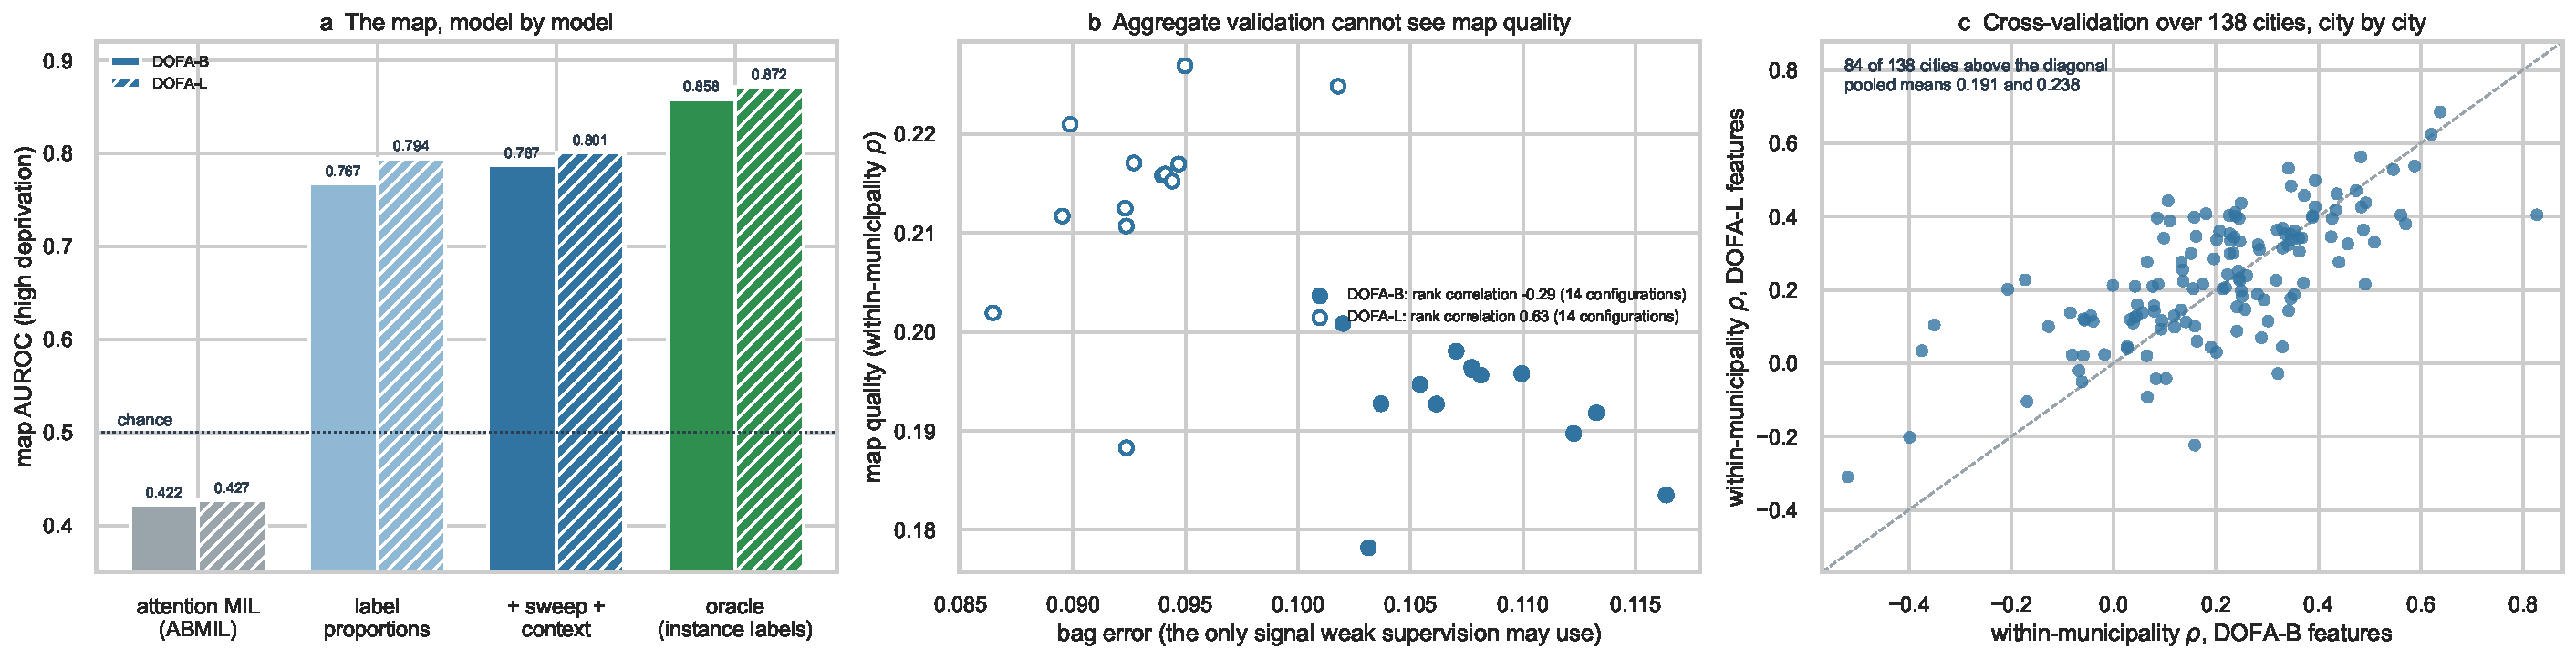
\includegraphics[width=\linewidth]{fig3_dissociation.pdf}
\caption{\textbf{Bag prediction versus localization.}
\textbf{a}, Map quality by model family on identical features and labels, DOFA base
solid and DOFA large hatched; the first three families are measured on the national-set
pool, the swept head on the expanded pool of Fig.~2. Attention pooling solves the bag task from the feature mean and receives no
localization gradient; predicting instances and averaging predictions makes the map the
mechanism. \textbf{b}, Across the fourteen sweep configurations (grouped training
folds of the national set), the only criterion weak supervision may monitor is nearly
uncorrelated with within-municipality map quality, and positively correlated
($+0.62$) with the pooled AUROC it would seem to proxy.}
\label{fig:dissociation}
\end{figure}

Reversing the order of prediction and aggregation removes the failure. Predicting every
token and averaging the predictions (deep learning from label
proportions~\cite{quadrianto2009,ardehaly2017,dulac2019}) ties the training signal
directly to the token scores that form the map: AUROC 0.761 (DOFA base) and 0.782
(DOFA large) under the same features, bags and labels on that national-set pool, and
0.802 with either backbone for the swept head with 480 m of neighborhood context on the
expanded pool of Fig.~\ref{fig:curve}. Because
Mexican municipal grades are population-weighted aggregates of tract grades, the setting
is label proportions with \emph{known} instance weights; weighting each token by its
tract's census population is a robustness variant that performs equivalently
($\rho = 0.232$ against $0.227$ on validation and $0.182$ against $0.196$ on test with
DOFA base; $0.242$ against $0.242$ and $0.253$ against $0.226$ with DOFA large).

The sweep also quantified a limitation of model selection under weak supervision.
Across the fourteen configurations, bag-level error, the only selection signal weak
supervision may legitimately use, has a rank correlation of $-0.14$ with
within-municipality map quality and $+0.62$ with the map's pooled AUROC, the wrong sign
for a selection criterion (Fig.~\ref{fig:dissociation}b). Fourteen configurations give
these correlations a standard error near $0.27$, so the estimate is coarse; what it
supports is that selection on bag error is close to uninformative about the quantity
that matters. Whether this extends beyond settings where the bag label is an average of
instance states is open, but any pipeline whose product is the map is affected,
computational pathology included, which is why the benchmark includes held-out instance
labels.

\subsection{External validity}

We ran four independent comparisons to test whether the map measures deprivation or a
pipeline artifact (Fig.~\ref{fig:validation}). Against the leading downloadable product, Meta's Relative
Wealth Index~\cite{chi2022}, scored per tract on an identical universe
with a city-clustered bootstrap of the paired difference (2{,}958 shared AGEB), the map
wins in 18 of 22 municipalities with either backbone: $\Delta\rho = +0.22$ [$+0.08,
+0.29$] for DOFA base and $+0.22$ [$+0.10$, $+0.29$] for DOFA large; on the test cities
the differences are $+0.13$ [$-0.07, +0.26$] and $+0.16$ [$-0.02$, $+0.29$],
directionally consistent and not individually significant over 22 municipalities
(Fig.~\ref{fig:validation}a). A
land-cover-plus-NDVI head with no learned representation reaches $\rho = 0.150$ on
validation and $0.219$ on test, where it is statistically indistinguishable from the
full model with either backbone (paired $\Delta\rho = -0.02$ [$-0.18$, $+0.10$] for
DOFA base, winning 16 of 29 municipalities; $+0.01$ [$-0.10$, $+0.11$] for DOFA large,
winning 18). The learned features' advantage within municipalities is
therefore split-dependent; what holds on both splits is their edge on the bag task (bag
error 0.095 against 0.110) and, on test, on high-deprivation detection (AUROC 0.821
against 0.781). Much of the within-municipality ordering is captured by land cover
alone. This is consistent with the exchange rate, which measures what the published
supervision recovers for a fixed feature set, whichever encoder produces it. Against an index from an institution whose data never entered training (CONAPO's
continuous urban marginalization index, built from a different indicator set over the
same census), the map correlates at $\rho = 0.361 \pm 0.073$ within municipalities on
validation and $0.257 \pm 0.146$ on test with DOFA base, and at $0.341 \pm 0.053$ and
$0.313 \pm 0.113$ with DOFA large, in every case at least as high as against its own
five-level training construct, consistent with the continuous index resolving ties that
five levels cannot (Fig.~\ref{fig:validation}b). In simulated
geographic targeting with fractional funding of the marginal tract, allocating by the
map instead of the municipal aggregate closes 26--43\% of the gap to census-guided
allocation on validation at budgets of 10\% and above and 31--66\% on the test cities
with DOFA base, and 31--38\% and 42--64\% with DOFA large, with no crossover on test
for either (Fig.~\ref{fig:validation}c). At the tightest validation budget (5\%), where
errors at the top of the ranking are most costly, DOFA base loses to the aggregate and
DOFA large closes 4\% of the gap. The map is also not an administrative
artifact. Crossing a municipal border where deprivation does not change moves it by
$+0.019$ [$-0.002$, $+0.155$] with DOFA base and $-0.003$ [$-0.033$, $+0.126$] with
DOFA large, and tract borders inside municipalities are crossed smoothly ($+0.001$ and
$-0.004$). An earlier $+0.14$ border jump traced to bag-limited neighborhood
adjacency at inference and disappeared after the adjacency was computed city-wide. The
test cities contain too few same-grade cross-border pairs to repeat this control there.

\begin{figure}[htbp]
\centering
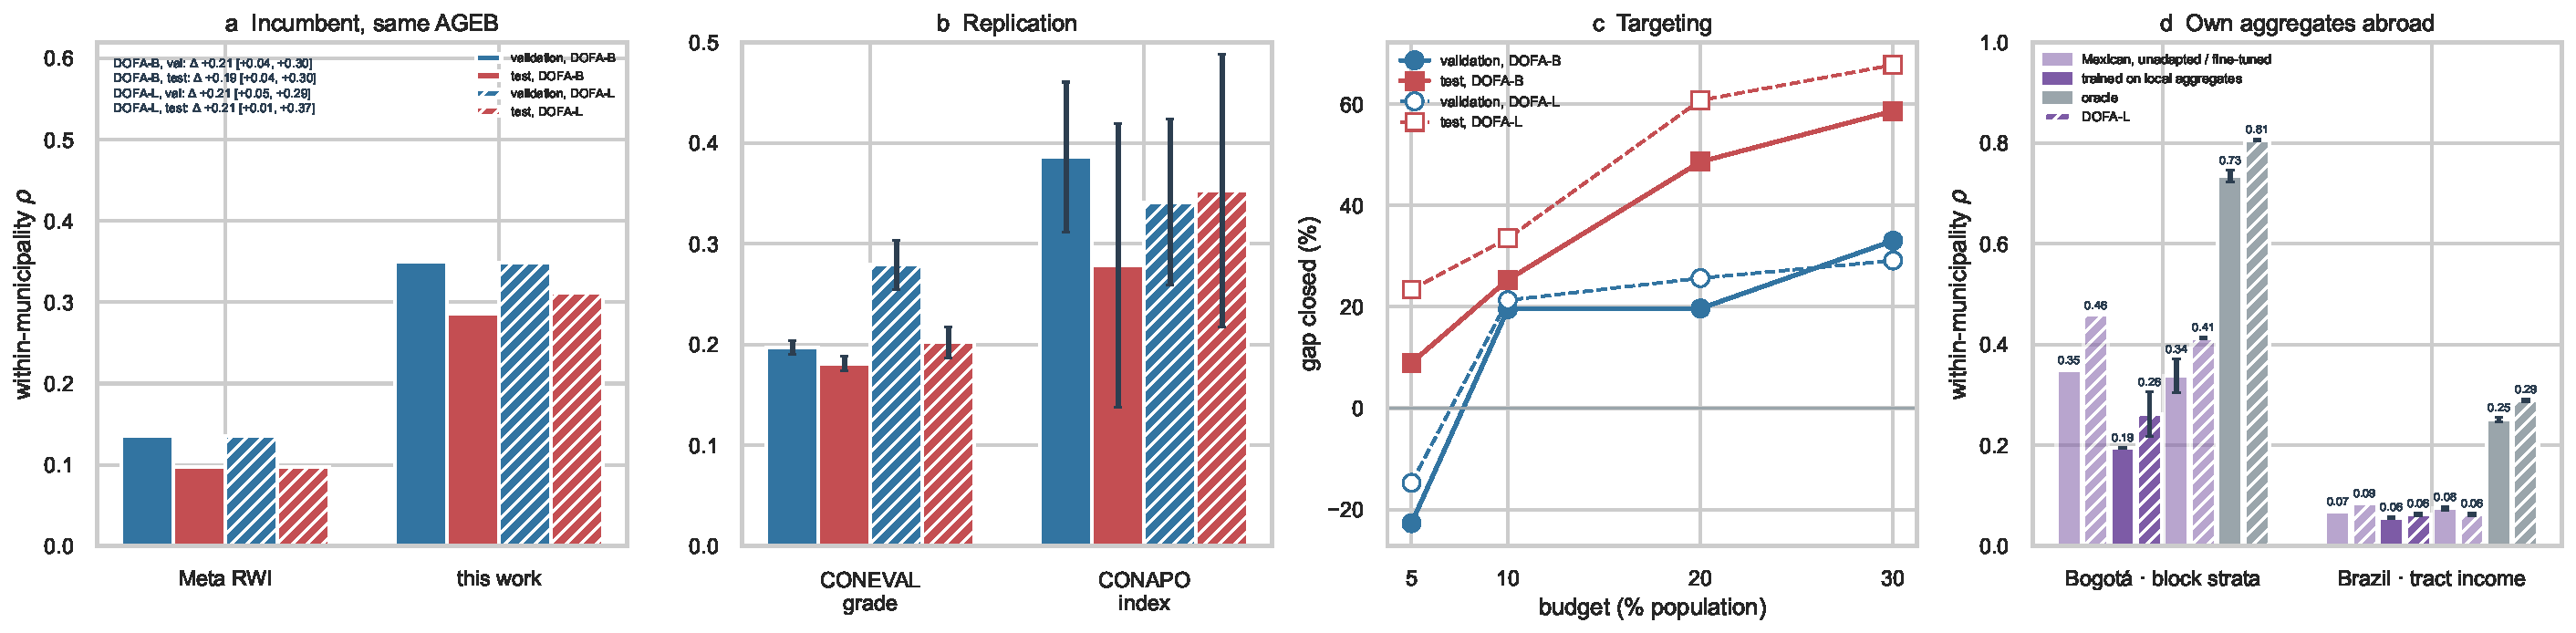
\includegraphics[width=\linewidth]{fig4_validation.pdf}
\caption{\textbf{External validity.} Blue, validation; red, held-out test;
purple in \textbf{d}, which belongs to neither split; DOFA base solid and filled, DOFA
large hatched or hollow. \textbf{a}, Within-municipality agreement on the identical AGEB
universe reached by the incumbent's grid; annotation, city-clustered bootstraps of the
paired difference per split. \textbf{b}, Replication against an independent
institution's continuous index, beside the map's agreement with the construct it was
trained toward (error bars: s.d. over seeds on the CONEVAL bars, city-clustered bootstrap
half-widths on the CONAPO bars).
\textbf{c}, Share of the aggregate-to-census targeting gap closed at each budget,
people pooled per split; validation loses at the tightest budget, test does not.
\textbf{d}, Transfer under each country's own aggregates: within-municipality $\rho$
against Bogot\'a's block strata (35 bags; $n = 12{,}738$ built tokens) and against
tract median income across 47 Brazilian municipalities (48 bags; $n = 110{,}728$), for
the Mexican model unadapted, the head trained from scratch on the local municipal
aggregates, the Mexican heads fine-tuned on them, and the fully supervised oracle; bars
are means over three seeds with their s.d. where seeds apply, under grouped folds by
municipality (Bogot\'a's oracle: spatial folds).}
\label{fig:validation}
\end{figure}

The sharper version of the question is what a practitioner would get for free. Four global
products were scored on the identical universe under the identical protocol
(Fig.~\ref{fig:incumbents}a, Table~\ref{tab:products}). Against GHSL residential
population the map wins clearly, $\Delta\rho = +0.29$ [$-0.00$, $+0.50$] on validation
and $+0.19$ [$+0.05$, $+0.29$] on test with DOFA base, $+0.29$ [$+0.02$, $+0.46$] and
$+0.22$ [$+0.07$, $+0.37$] with DOFA large, the only one of the four that separates on
test. Against GHSL built-up surface ($+0.15$ [$-0.10$, $+0.30$]; $+0.06$ [$-0.10$,
$+0.16$] with DOFA base) and GHSL building height ($+0.13$ [$-0.10$, $+0.29$]; $+0.11$
[$-0.06$, $+0.23$]) the map leads on both splits and both backbones, winning 14 to 16 of
22 municipalities on test, with intervals that include zero throughout. Against
nighttime lights the two are tied: $+0.04$ [$-0.11$, $+0.15$] on validation and $-0.04$
[$-0.25$, $+0.10$] on test with DOFA base, $+0.04$ [$-0.09$, $+0.13$] and $+0.00$
[$-0.18$, $+0.13$] with DOFA large. A 1 km light product, free and requiring no model,
orders tracts inside a Mexican municipality about as well as the maps do. That comparison is handicapped in the light product's disfavor by resolution, since
63\% of test tracts are smaller than one of its cells and take the value at an interior
point, and it is reported at face value regardless: within the precision fourteen
cities allow, we cannot show the map beats nighttime lights.

\begin{figure}[htbp]
\centering
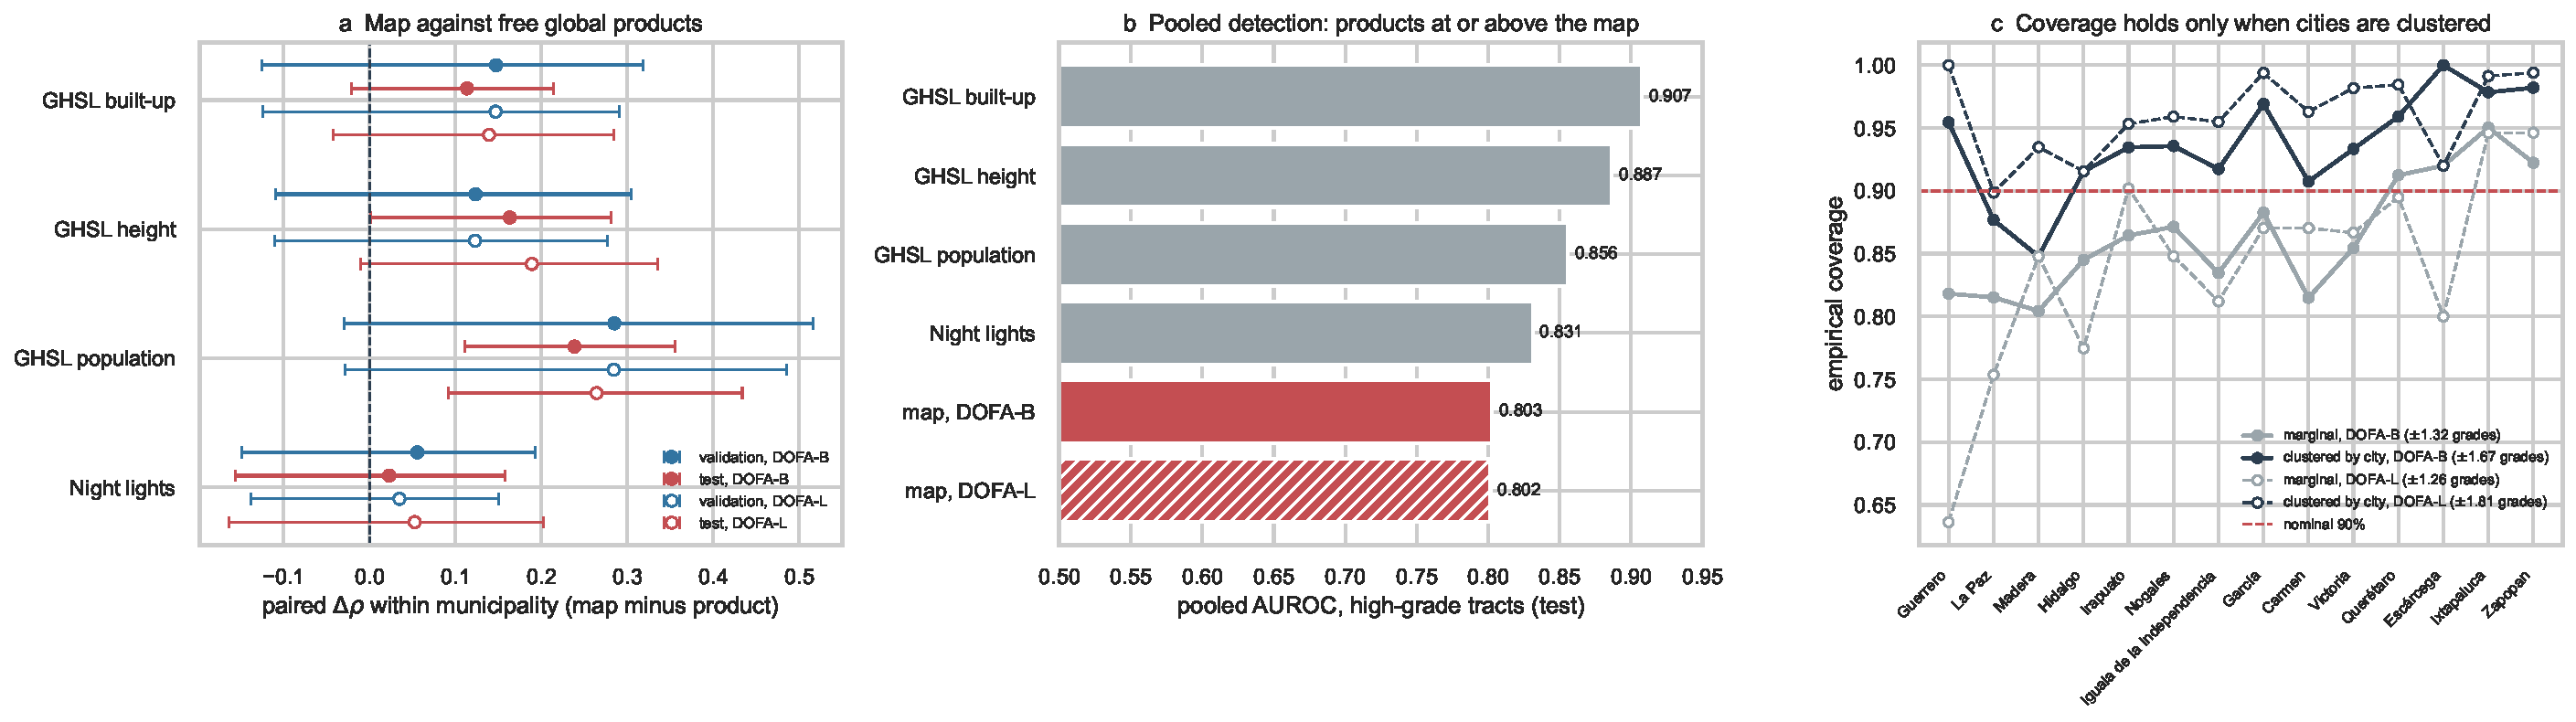
\includegraphics[width=\linewidth]{fig5_incumbents.pdf}
\caption{\textbf{Free products, and the confidence the map can carry.}
\textbf{a}, Paired within-municipality difference between the map and each downloadable
global product on the identical tract universe, blue validation and red test, filled
DOFA base and hollow DOFA large, with city-clustered bootstrap intervals; only gridded population separates from the map on
test, and nighttime lights straddle zero on both splits. \textbf{b}, Pooled detection of
high and very-high grade tracts across the test cities: all four products land at or
above the map, which is the bag-versus-map dissociation of Fig.~3 arriving on external ground.
\textbf{c}, Conformal coverage per test city at 90\% nominal, calibrated on the
validation cities, DOFA base solid and DOFA large dashed. The marginal rule falls below
nominal in ten of fourteen cities with DOFA base and eleven with DOFA large; the
clustered rule restores coverage at a half-width of 1.68 and 1.85 of the five grades.}
\label{fig:incumbents}
\end{figure}

\begin{table}[htbp]
\centering
\caption{Free global products under the map's own protocol, for both backbones.
Within-$\rho$ is the mean over municipalities of the within-municipality Spearman
correlation against the held-out tract grade, on the identical universe; $\Delta$ is the
paired difference, map minus product, with a city-clustered bootstrap interval; AUROC is
pooled detection of high and very-high grade tracts across the split (map with DOFA base
0.828 on validation and 0.829 on test, with DOFA large 0.818 and 0.827). Orientation was
fixed before measurement: deprivation is the negative of every product. The
nighttime-light row rests on interior-point sampling for 63\% of tracts, which are
smaller than one of its 30 arcsec cells.}
\small
\resizebox{\linewidth}{!}{%
\begin{tabular}{llcccccc}
\toprule
 & & & \multicolumn{2}{c}{DOFA base} & \multicolumn{2}{c}{DOFA large} & \\
\cmidrule(lr){4-5}\cmidrule(lr){6-7}
Product & Split & Product $\rho$ & Map $\rho$ & $\Delta$ [95\% CI] & Map $\rho$ & $\Delta$ [95\% CI] & AUROC product\\
\midrule
GHSL built-up surface & val & 0.202 & 0.354 & $+0.152$ [$-0.103$, $+0.303$] & 0.354 & $+0.152$ [$-0.085$, $+0.268$] & 0.866\\
 & test & 0.174 & 0.232 & $+0.059$ [$-0.098$, $+0.160$] & 0.267 & $+0.093$ [$-0.078$, $+0.218$] & 0.908\\
GHSL building height & val & 0.226 & 0.354 & $+0.128$ [$-0.096$, $+0.291$] & 0.354 & $+0.128$ [$-0.068$, $+0.245$] & 0.859\\
 & test & 0.119 & 0.232 & $+0.113$ [$-0.062$, $+0.233$] & 0.267 & $+0.148$ [$-0.037$, $+0.278$] & 0.886\\
GHSL population & val & 0.065 & 0.354 & $+0.289$ [$-0.001$, $+0.497$] & 0.354 & $+0.290$ [$+0.022$, $+0.460$] & 0.872\\
 & test & 0.045 & 0.232 & $+0.188$ [$+0.051$, $+0.289$] & 0.267 & $+0.222$ [$+0.066$, $+0.366$] & 0.855\\
Nighttime lights & val & 0.327 & 0.364 & $+0.037$ [$-0.109$, $+0.149$] & 0.363 & $+0.036$ [$-0.093$, $+0.125$] & 0.840\\
 & test & 0.249 & 0.210 & $-0.039$ [$-0.245$, $+0.104$] & 0.252 & $+0.002$ [$-0.178$, $+0.126$] & 0.831\\
\bottomrule
\end{tabular}}
\label{tab:products}
\end{table}

The pooled comparison points the other way, and in doing so repeats the dissociation of
the previous section on external ground. For detecting high and very-high grade tracts
across the whole test set, all four products land at or above the map: built-up surface
reaches AUROC 0.908, building height 0.886, population 0.855 and nighttime lights 0.831,
against the map's 0.829 with DOFA base and 0.827 with DOFA large
(Fig.~\ref{fig:incumbents}b). The products carry more of the national gradient, which is the
easy half of the problem and the half gridded global layers are built for. What the
supervision buys, where it buys anything, is the ordering inside a municipality, the half
a targeting decision needs and the half no global product was built to deliver.

The products that match the map as competitors were also offered to it as inputs. With
full tract supervision the four GHSL and light columns lift the standardized oracle from
$\rho = 0.261$ to $0.291$ on validation (paired difference $+0.030$ [$+0.011$,
$+0.050$] over 36 municipalities); the WorldCover fractions add $+0.014$ [$-0.004$,
$+0.030$], and both together $+0.030$ [$+0.012$, $+0.046$]. Under municipal
supervision none of it reaches the map. Early fusion gives $0.225$ with the GHSL and
light columns, $0.212$ with WorldCover and $0.221$ with both, against the canonical
$0.227$; late fusion, which hands the columns their own scoring weights, gives $0.210$
and $0.226$ (Table~\ref{tab:inputs}). Information that a tract-supervised head
extracts from four columns is invisible to a gradient carried by a few hundred bag
labels, and a dedicated pathway makes it worse rather than better, consistent with the
rurality shortcut: built surface and population explain the municipal label well, the
head leans on them, and the ordering inside the municipality degrades.

\begin{table}[htbp]
\centering
\caption{Global products offered to the model as input features, validation cities,
within-municipality Spearman, three seeds. GHSL built-up surface, building height,
population and nighttime lights as four token columns; WorldCover as its eleven class
fractions plus NDVI mean and dispersion. The oracle rows are standardized, with their
own no-extras reference; the paired difference is per municipality, seed-averaged, with a
city-clustered bootstrap. The map rows fuse the columns either into the projection
(early) or straight into the scoring layer (late).}
\begin{tabular}{llccc}
\toprule
Head & Extra inputs & Seeds & Mean & Paired difference [95\%]\\
\midrule
Oracle & none (reference) & 0.288 / 0.239 / 0.257 & 0.261 & \\
Oracle & WorldCover & 0.288 / 0.261 / 0.272 & 0.274 & $+0.014$ [$-0.004$, $+0.030$]\\
Oracle & GHSL + lights & 0.293 / 0.281 / 0.298 & 0.291 & $+0.030$ [$+0.011$, $+0.050$]\\
Oracle & both & 0.291 / 0.278 / 0.300 & 0.289 & $+0.030$ [$+0.012$, $+0.046$]\\
\midrule
Map & none (canonical) & 0.242 / 0.224 / 0.215 & 0.227 & \\
Map, early & WorldCover & 0.207 / 0.221 / 0.209 & 0.212 & \\
Map, early & GHSL + lights & 0.226 / 0.236 / 0.214 & 0.225 & \\
Map, early & both & 0.220 / 0.227 / 0.217 & 0.221 & \\
Map, late & GHSL + lights & 0.214 / 0.217 / 0.198 & 0.210 & \\
Map, late & both & 0.241 / 0.221 / 0.216 & 0.226 & \\
\bottomrule
\end{tabular}
\label{tab:inputs}
\end{table}

\subsection{Transfer to Colombia and Brazil}

Applied unchanged to Bogot\'a, the model orders Colombia's block-level socioeconomic
strata at $\rho = 0.318$ (AUROC 0.716 for the deprived strata 1--2 over 14{,}132 tokens
joined to blocks; Fig.~\ref{fig:validation}d). Applied to Rio de Janeiro, it detects
IBGE's mapped informal settlements barely above chance (AUROC 0.557 among built-up
tokens; Fig.~\ref{fig:validation}d). The two targets differ in construct: Colombian strata measure the same graded
deprivation ordering as the GRS over the whole urban fabric, while the AGSN mask
delimits informality, a partly orthogonal notion. The model learned a deprivation
gradient from the aggregates, and that gradient transfers across countries; informality
detection does not follow from it.

Repeating the design on each country's own aggregates asks whether the Mexican result is
a property of the method or of Mexico (Fig.~\ref{fig:validation}d,
Table~\ref{tab:transfer}). Trained from scratch on Colombia's municipal poverty rate over 35 bags, the
head orders Bogot\'a's block strata at $\rho = 0.21$ (seeds $0.22$, $0.18$, $0.24$;
AUROC 0.63 for the most deprived quartile), against $0.31$ for the Mexican model applied
unchanged to the same built tokens and $0.25$ for the Mexican heads fine-tuned on the
Colombian aggregates ($0.29$, $0.14$, $0.31$, the least stable row). Trained on
Brazil's municipal mean income over 48 bags, it orders tract median income within
municipalities at $\rho = 0.12$ [$0.07$, $0.17$] over 47 municipalities ($0.11$,
$0.12$, $0.13$; pooled $0.33$; AUROC 0.64), against $0.10$ [$0.05$, $0.15$] zero-shot
and $0.08$ for the fine-tuned Mexican heads. The fully supervised references are
$0.75$ in Bogot\'a under spatial folds (AUROC 0.91) and $0.25$ [$0.20$, $0.30$] in
Brazil under municipal folds. Both countries land where the Mexican curve places a
supply of a few dozen bags ($\rho \approx 0.15$ at fifty), and Brazil's aggregate
is a mean income rather than a graded deprivation share, a weaker match to the head. The
method replicates on labels of a different construct from a different office; what the
two countries lack at this stage is the supply of aggregates, which is the axis the
curve measures.

\begin{table}[htbp]
\centering
\caption{Transfer under each country's own municipal aggregates (Fig.~\ref{fig:validation}d).
Within-municipality Spearman against the fine truth, grouped five-fold by municipality,
per seed; Bogot\'a's oracle folds over 3.2 km spatial cells. Colombia: 35 bags, the
Bogot\'a block strata as truth over 12{,}738 built tokens. Brazil: 48 bags, tract median
income of the household head as truth over 110{,}728 tokens in 47 municipalities, with
the municipality-bootstrap interval of the mean. AUROC is for the most deprived quartile
of the truth, pooled. The earlier zero-shot protocol, without the built-token filter,
gave $\rho = 0.318$ and AUROC 0.716 (strata 1--2) in Bogot\'a over 14{,}132 tokens and
AUROC 0.557 for Rio's mapped informal settlements over 34{,}331 built tokens.}
\begin{tabular}{llcccc}
\toprule
Country & Method & Seeds & Mean [95\%] & Pooled $\rho$ & AUROC\\
\midrule
Colombia & Mexican, unadapted & 0.311 & 0.311 & 0.311 & 0.705\\
Colombia & local aggregates & 0.223 / 0.178 / 0.238 & 0.213 & 0.213 & 0.630\\
Colombia & Mexican, fine-tuned & 0.294 / 0.138 / 0.305 & 0.246 & 0.246 & 0.660\\
Colombia & oracle & 0.741 / 0.758 / 0.749 & 0.749 & 0.749 & 0.906\\
\midrule
Brazil & Mexican, unadapted & 0.099 & 0.099 [0.048, 0.148] & 0.283 & 0.648\\
Brazil & local aggregates & 0.115 / 0.119 / 0.130 & 0.121 [0.074, 0.171] & 0.332 & 0.636\\
Brazil & Mexican, fine-tuned & 0.074 / 0.077 / 0.084 & 0.078 [0.026, 0.129] & 0.337 & 0.633\\
Brazil & oracle & 0.239 / 0.269 / 0.234 & 0.247 [0.197, 0.297] & 0.472 & 0.704\\
\bottomrule
\end{tabular}
\label{tab:transfer}
\end{table}

\subsection{Uncertainty and limits}

A map offered for targeting has to say where it is unsure. The ensemble of three seeds
supplies the obvious candidate, and it does not work. Seed disagreement ranks the tract
errors at $\rho = 0.084$ [$0.002$, $0.140$] within municipalities on validation and
$0.044$ [$-0.011$, $0.084$] on test with DOFA base, and at $0.115$ [$0.045$, $0.187$] and
$0.079$ [$0.030$, $0.120$] with DOFA large: a signal too weak to act on. Acting on it
anyway buys nothing. Setting aside the least confident tracts inside each municipality,
over a panel of municipalities held fixed at every depth so attrition cannot manufacture
a trend, leaves map quality flat or lower: $0.390$ to $0.369$ from no discard to half
discarded on validation and $0.317$ to $0.327$ on test with DOFA base, $0.382$ to
$0.346$ and $0.316$ to $0.274$ with DOFA large, every point inside every other point's
interval. (These are tract-mean correlations, higher than
the token-level figures quoted above because averaging tokens to tracts removes noise; the
comparison here is internal, so the estimator only has to be consistent with itself.)
Ensembling over seeds does not produce an uncertainty layer for this problem, and we
report no confidence raster.

What can be attached is an interval. Split conformal calibrated on the validation cities
and evaluated on the test cities~\cite{vovk2005} gives, at 90\% nominal coverage, a
half-width of 1.29 grades under the marginal rule with DOFA base (1.30 with DOFA large),
and that rule undercovers: 0.869 overall and below nominal in 10 of the 14 test cities,
worst at La Paz (0.768), with DOFA base; 0.857, 11 cities and Hidalgo (0.718) with DOFA
large. Pricing in that cities are not exchangeable with one another, by taking each
calibration city's own quantile and then the 90th percentile across cities, restores
coverage to 0.953 and 0.963 with one city below nominal, at the cost of a half-width of
1.68 and 1.85 grades (Fig.~\ref{fig:incumbents}c, Table~\ref{tab:conformal}). On a five-level scale
that interval spans most of the range. The honest statement is that the map orders
neighborhoods and cannot commit to a grade, and that any interval which ignores
between-city variation will be too narrow.

\begin{table}[htbp]
\centering
\caption{Conformal grade intervals at 90\% nominal coverage, calibrated on the validation
cities and evaluated on the test cities, for both backbones. The marginal rule assumes all
tracts exchangeable; the clustered rule takes each calibration city's quantile and then
the 90th percentile across cities.}
\begin{tabular}{llccccc}
\toprule
Backbone & Rule & Half-width (grades) & Coverage & Worst city & Worst city coverage & Cities below\\
\midrule
DOFA base & marginal & 1.29 & 0.869 & La Paz & 0.768 & 10 of 14\\
DOFA base & clustered by city & 1.68 & 0.953 & Madera & 0.870 & 1 of 14\\
DOFA large & marginal & 1.30 & 0.857 & Hidalgo & 0.718 & 11 of 14\\
DOFA large & clustered by city & 1.85 & 0.963 & La Paz & 0.899 & 1 of 14\\
\bottomrule
\end{tabular}
\label{tab:conformal}
\end{table}

The failures are concentrated and can be named (Table~\ref{tab:audit}). Ranking the
fourteen test cities by the within-municipality correlation their map achieves, the same
three sit at or below zero with either backbone: Guerrero, Chihuahua ($-0.51$ over 21
tracts with DOFA base, $-0.07$ with DOFA large), Ciudad del Carmen, Campeche ($-0.27$ and
$-0.21$ over 54), and Escárcega, Campeche ($-0.00$ and $-0.32$ over 24). All three are
small, and the top of the ranking is not: Iguala de la Independencia ($+0.64$ and $+0.66$
over 133 tracts), La Paz ($+0.53$ and $+0.43$ over 276), Irapuato ($+0.47$ and $+0.50$
over 214) and Ixtapaluca ($+0.47$ and $+0.41$ over 463). The pattern in the ranking is
tract count rather than deprivation share, which is the modifiable-areal-unit effect of
the Limits section arriving as a per-city failure mode: a municipality carved into two
dozen tracts offers too few ranks for the correlation to stabilize, and the map's
ordering inside it should not be used. Seed spread does not flag these cities either;
Guerrero's median spread (0.101 with DOFA base) sits at the middle of the fourteen.

\begin{table}[htbp]
\centering
\caption{The fourteen test cities ranked by the within-municipality correlation their map
achieves with DOFA base, worst first, with the DOFA large value beside it. Tract-mean
scores. Spread is the median across tracts of the standard deviation over three seeds,
which does not separate the failures from the successes.}
\begin{tabular}{lrrrrrr}
\toprule
 & & & \multicolumn{2}{c}{DOFA base} & \multicolumn{2}{c}{DOFA large}\\
\cmidrule(lr){4-5}\cmidrule(lr){6-7}
City & Municipalities & Tracts & Within-$\rho$ & Seed spread & Within-$\rho$ & Seed spread\\
\midrule
Guerrero & 1 & 21 & $-0.510$ & 0.101 & $-0.067$ & 0.185\\
Ciudad del Carmen & 1 & 54 & $-0.267$ & 0.069 & $-0.215$ & 0.127\\
Esc\'arcega & 1 & 24 & $-0.001$ & 0.093 & $-0.319$ & 0.117\\
Madera & 1 & 46 & $0.052$ & 0.133 & $0.154$ & 0.202\\
Quer\'etaro & 3 & 514 & $0.091$ & 0.109 & $0.284$ & 0.115\\
Zapopan & 2 & 335 & $0.105$ & 0.104 & $0.357$ & 0.120\\
Garc\'ia & 3 & 324 & $0.257$ & 0.088 & $0.163$ & 0.129\\
Nogales & 1 & 171 & $0.261$ & 0.093 & $0.329$ & 0.139\\
Victoria & 1 & 165 & $0.373$ & 0.102 & $0.458$ & 0.116\\
Hidalgo & 1 & 71 & $0.425$ & 0.098 & $0.234$ & 0.151\\
Irapuato & 1 & 214 & $0.465$ & 0.121 & $0.498$ & 0.103\\
Ixtapaluca & 4 & 463 & $0.471$ & 0.097 & $0.415$ & 0.151\\
La Paz & 1 & 276 & $0.534$ & 0.095 & $0.433$ & 0.115\\
Iguala de la Independencia & 1 & 133 & $0.639$ & 0.125 & $0.658$ & 0.187\\
\bottomrule
\end{tabular}
\label{tab:audit}
\end{table}

Beyond the named failures, three limits bound every claim. The upper bound itself is low: even with full tract labels and neighborhood context,
160 m tokens support $\rho = 0.251$ within municipalities on validation and $0.233$ on test
with DOFA base, $0.318$ and $0.295$ with DOFA large: sufficient to order neighborhoods,
too coarse to resolve individual blocks. Agreement depends strongly on tract size with
either backbone: $\rho = 0.26$ for tracts covered by 1--3 tokens ($0.18$ with DOFA
large), rising to $0.43$ at 20--49
tokens, and collapsing to $0.13$ in the two municipalities dominated by very large
tracts; the test split reproduces the pattern noisily, peaking at $0.38$ and collapsing
in its single large-tract municipality. This is the modifiable areal unit problem,
quantified here by tract size (Table~\ref{tab:maup}). Ecological caution applies throughout: the model recovers where deprived tracts are, and
tract grades are themselves aggregates over households; neither the labels nor the maps
identify deprived households, and the targeting simulation counts the population of
deprived tracts; deprived individuals themselves are unobserved.

\begin{table}[htbp]
\centering
\caption{Agreement by tract size on the validation cities. Within-municipality Spearman
$\rho$ of tract-mean scores over municipalities with at least ten tracts in the bin, for
both backbones.}
\begin{tabular}{rrrrcc}
\toprule
Tokens per tract & Tracts & Median population & Municipalities & DOFA base & DOFA large\\
\midrule
1--3 & 567 & 211 & 15 & 0.257 & 0.183\\
4--9 & 849 & 1{,}948 & 16 & 0.338 & 0.378\\
10--19 & 999 & 2{,}644 & 20 & 0.352 & 0.355\\
20--49 & 464 & 3{,}231 & 14 & 0.432 & 0.374\\
$\geq$50 & 79 & 3{,}561 & 2 & 0.127 & 0.094\\
\bottomrule
\end{tabular}
\label{tab:maup}
\end{table}

\section{Discussion}

Prior applications of this technology predict aggregates across space; the exchange
rate measures how much sub-municipal detail can be recovered from statistics published
at a given resolution, which is the question a statistics office would ask. In
operational terms: the national supply of municipal aggregates recovers 84--90\% of
what DOFA base features support and 76--77\% of what DOFA large features support,
coarser publication reduces recovery in proportion, and sensor content rather than
resolution is the binding property. A larger backbone raises the fully supervised bound
by $0.06$ and the map by $0.02$ to $0.03$, on both splits and under cross-validation over
all 138 cities: the representation is one limit on the map and the supply of labels is
the larger one. The targeting experiment
expresses the result as people reached, including the one budget where the map
underperforms the aggregate. Three negative results matter for similar efforts:
attention-based pooling fails for a structural reason, selection on aggregate error is
close to uninformative about map quality, and informality detection does not follow
from a deprivation gradient. All three will recur in other weakly supervised mapping
work.

The comparison against free global grids sets the operational recommendation more
honestly than an accuracy table would. On the pooled task every downloadable product
outperforms the map, and within municipalities only the population grid separates from it
on test, with nighttime lights matching it on both splits, and offering the grids to the
model as inputs raises the fully supervised bound without moving the weakly supervised
map. So where the question is which
municipalities are poor, a global layer answers it today at no cost; where the question is
which neighborhoods inside a municipality are poorest, the aggregate-trained map is the
better instrument, by a margin smaller than the enthusiasm in this literature would
suggest. The missing uncertainty layer sharpens the same point. Seeds disagree where the
map is right about as often as where it is wrong, and the interval that does hold its
coverage across cities spans 1.7 to 1.9 of the five grades. What this method supports publishing
is a ranking with the small municipalities named and excluded; a graded raster would
overstate it.

Mexico's dual-level publication made the calibration possible, and the Colombian and
Brazilian rows test the extrapolation the paper invites: a country that publishes only
municipal aggregates, of a construct and an office of its own, recovers a
within-municipality ordering from them, at the level the Mexican curve assigns to a
supply of a few dozen bags. The two countries hold 1{,}122 and 5{,}570 labelled
municipalities; walking their curves toward the Mexican supply is the measurement that
follows, and every number here is reproducible from the released frozen features.

\section{Conclusions}

Municipal aggregates, the level at which most countries actually publish social
statistics, carry most of the neighborhood-scale ordering that frozen satellite features
support: 84\% of the fully supervised upper bound on unseen test cities and 90\% on
validation with DOFA base, 77\% and 76\% with DOFA large, whose maps are higher in
absolute terms ($\rho = 0.23$ against $0.20$ on test). The upper bound itself is low
($\rho = 0.23$ to $0.30$ within municipalities at 160 m), which bounds every claim in
this paper and, we would argue, every claim in this setting built on free decametric
imagery. Within that bound, the supervision-efficiency
analysis is operational for statistics offices: a few hundred aggregates recover most of
what the full national supply does, coarser publication forfeits recovery in proportion,
and sensor content matters more than resolution. Two methodological results travel
beyond the application: attention-based multiple-instance learning produces chance-level
maps whenever the bag task is solvable from the feature mean, and model selection on
bag-level error is close to uninformative about map quality, which argues for benchmarks
with held-out instance labels wherever maps are the product. A third caution is
operational: measured against the free global grids a practitioner already has, the map's
advantage is confined to the within-municipality ordering and is resolvable on fourteen
test cities only against gridded population, while ensembling supplies no uncertainty
layer and an honest grade interval spans 1.7 to 1.9 of the five levels. The design repeats
outside Mexico on each country's own municipal aggregates, in Colombia and Brazil, at
the recovery the curve predicts for their present supply of bags. All data, frozen
features, labels, splits and code are released.

\begin{thebibliography}{10}
\bibitem{jean2016} Jean, N. \emph{et al.} Combining satellite imagery and machine
learning to predict poverty. \emph{Science} \textbf{353}, 790--794 (2016).
\bibitem{yeh2020} Yeh, C. \emph{et al.} Using publicly available satellite imagery and
deep learning to understand economic well-being in Africa. \emph{Nat. Commun.}
\textbf{11}, 2583 (2020).
\bibitem{chi2022} Chi, G., Fang, H., Chatterjee, S. \& Blumenstock, J. E. Microestimates
of wealth for all low- and middle-income countries. \emph{Proc. Natl Acad. Sci. USA}
\textbf{119}, e2113658119 (2022).
\bibitem{burke2021} Burke, M., Driscoll, A., Lobell, D. B. \& Ermon, S. Using satellite
imagery to understand and promote sustainable development. \emph{Science} \textbf{371},
eabe8628 (2021).
\bibitem{head2017} Head, A., Manguin, M., Tran, N. \& Blumenstock, J. E. Can human
development be measured with satellite imagery? \emph{Proc. ICTD} 8 (2017).
\bibitem{engstrom2022} Engstrom, R., Hersh, J. \& Newhouse, D. Poverty from space: using
high resolution satellite imagery for estimating economic well-being. \emph{World Bank
Econ. Rev.} \textbf{36}, 382--412 (2022).
\bibitem{ayush2021} Ayush, K., Uzkent, B., Tanmay, K., Burke, M., Lobell, D. \& Ermon, S.
Efficient poverty mapping from high resolution remote sensing images. \emph{Proc. AAAI}
\textbf{35}, 12--20 (2021).
\bibitem{rolf2021} Rolf, E. \emph{et al.} A generalizable and accessible approach to
machine learning with global satellite imagery. \emph{Nat. Commun.} \textbf{12}, 4392
(2021).
\bibitem{lee2022} Lee, K. \& Braithwaite, J. High-resolution poverty maps in Sub-Saharan
Africa. \emph{World Dev.} \textbf{159}, 106028 (2022).
\bibitem{aiken2022} Aiken, E., Bellue, S., Karlan, D., Udry, C. \& Blumenstock, J. E.
Machine learning and phone data can improve targeting of humanitarian aid.
\emph{Nature} \textbf{603}, 864--870 (2022).
\bibitem{kuffer2016} Kuffer, M., Pfeffer, K. \& Sliuzas, R. Slums from space: 15 years
of slum mapping using remote sensing. \emph{Remote Sens.} \textbf{8}, 455 (2016).
\bibitem{stevens2015} Stevens, F. R., Gaughan, A. E., Linard, C. \& Tatem, A. J.
Disaggregating census data for population mapping using random forests with
remotely-sensed and ancillary data. \emph{PLoS ONE} \textbf{10}, e0107042 (2015).
\bibitem{wardrop2018} Wardrop, N. A. \emph{et al.} Spatially disaggregated population
estimates in the absence of national population and housing census data. \emph{Proc.
Natl Acad. Sci. USA} \textbf{115}, 3529--3537 (2018).
\bibitem{openshaw1984} Openshaw, S. \emph{The Modifiable Areal Unit Problem}. Concepts
and Techniques in Modern Geography 38 (Geo Books, Norwich, 1984).
\bibitem{carbonneau2018} Carbonneau, M.-A., Cheplygina, V., Granger, E. \& Gagnon, G.
Multiple instance learning: a survey of problem characteristics and applications.
\emph{Pattern Recognit.} \textbf{77}, 329--353 (2018).
\bibitem{yu2013} Yu, F. X., Liu, D., Kumar, S., Jebara, T. \& Chang, S.-F. $\propto$SVM
for learning with label proportions. \emph{Proc. ICML} 504--512 (2013).
\bibitem{wang2020} Wang, S., Chen, W., Xie, S. M., Azzari, G. \& Lobell, D. B. Weakly
supervised deep learning for segmentation of remote sensing imagery. \emph{Remote Sens.}
\textbf{12}, 207 (2020).
\bibitem{cong2022} Cong, Y. \emph{et al.} SatMAE: pre-training transformers for temporal
and multi-spectral satellite imagery. \emph{Adv. Neural Inf. Process. Syst.} \textbf{35}
(2022).
\bibitem{wang2023} Wang, Y. \emph{et al.} SSL4EO-S12: a large-scale multimodal,
multitemporal dataset for self-supervised learning in Earth observation. \emph{IEEE
Geosci. Remote Sens. Mag.} \textbf{11}, 98--106 (2023).
\bibitem{coneval2020} CONEVAL. Grado de Rezago Social por AGEB urbana 2020.
\url{https://www.coneval.org.mx/Medicion/IRS} (2021; accessed August 2026).
\bibitem{conapo2020} CONAPO. \'Indice de marginaci\'on urbana 2020.
\url{https://www.gob.mx/conapo/documentos/indices-de-marginacion-2020-284372} (2021;
accessed August 2026).
\bibitem{ilse2018} Ilse, M., Tomczak, J. M. \& Welling, M. Attention-based deep multiple
instance learning. \emph{Proc. ICML} 2127--2136 (2018).
\bibitem{lu2021} Lu, M. Y. \emph{et al.} Data-efficient and weakly supervised
computational pathology on whole-slide images. \emph{Nat. Biomed. Eng.} \textbf{5},
555--570 (2021).
\bibitem{quadrianto2009} Quadrianto, N., Smola, A. J., Caetano, T. S. \& Le, Q. V.
Estimating labels from label proportions. \emph{J. Mach. Learn. Res.} \textbf{10},
2349--2374 (2009).
\bibitem{ardehaly2017} Ardehaly, E. M. \& Culotta, A. Co-training for demographic
classification using deep learning from label proportions. \emph{Proc. ICDM Workshops}
1017--1024 (2017).
\bibitem{dulac2019} Dulac-Arnold, G., Zeghidour, N., Cuturi, M., Beyer, L. \& Vert,
J.-P. Deep multi-class learning from label proportions. \emph{arXiv:1905.12909} (2019).
\bibitem{xiong2024} Xiong, Z. \emph{et al.} Neural plasticity-inspired multimodal
foundation model for Earth observation. \emph{arXiv:2403.15356} (2024).
\bibitem{wang2025cfm} Wang, Y. \emph{et al.} Towards a unified Copernicus foundation
model for Earth vision. \emph{arXiv:2503.11849} (2025).
\bibitem{worldcover} Zanaga, D. \emph{et al.} ESA WorldCover 10 m 2020 v100. Zenodo
\url{https://doi.org/10.5281/zenodo.5571936} (2021).
\bibitem{ghsl2023} Pesaresi, M. \& Politis, P. GHS-BUILT-S and GHS-BUILT-H R2023A, and
Schiavina, M., Freire, S. \& MacManus, K. GHS-POP R2023A. European Commission, Joint
Research Centre \url{https://human-settlement.emergency.copernicus.eu/} (2023; accessed
September 2026).
\bibitem{li2020} Li, X., Zhou, Y., Zhao, M. \& Zhao, X. A harmonized global nighttime
light dataset 1992--2018. \emph{Sci. Data} \textbf{7}, 168 (2020). 2020 layer, Figshare
\url{https://doi.org/10.6084/m9.figshare.9828827}.
\bibitem{vovk2005} Vovk, V., Gammerman, A. \& Shafer, G. \emph{Algorithmic Learning in a
Random World} (Springer, 2005).
\bibitem{ibge2019} IBGE. Aglomerados subnormais 2019: classifica\c{c}\~ao preliminar.
\url{https://www.ibge.gov.br/geociencias/organizacao-do-territorio/tipologias-do-territorio/15788-aglomerados-subnormais.html}
(2020; accessed August 2026).
\bibitem{dane_ipm} DANE. Medida de pobreza multidimensional municipal de fuente censal
2018. Departamento Administrativo Nacional de Estad\'istica, Bogot\'a (2020).
\bibitem{mgn2023} DANE. Marco Geoestad\'istico Nacional 2023, nivel municipio.
\url{https://geoportal.dane.gov.co/} (2023; accessed September 2026).
\bibitem{ibge2022} IBGE. Censo Demogr\'afico 2022: agregados por setores censit\'arios e
por munic\'ipios, rendimento do respons\'avel.
\url{https://ftp.ibge.gov.br/Censos/Censo_Demografico_2022/} (2026; accessed September
2026).
\bibitem{bogota} Secretar\'ia Distrital de Planeaci\'on. Estratificaci\'on
socioecon\'omica urbana de Bogot\'a D.C. Datos Abiertos Bogot\'a
\url{https://datosabiertos.bogota.gov.co/dataset/estratificacion-para-bogota} (2024;
accessed August 2026).
\end{thebibliography}

\section*{Data availability}
The frozen benchmark (DOFA base and DOFA large vectors for every bag, municipal and
tract labels, splits, and the evaluation protocol) will be deposited on Zenodo with a
DOI at publication. All source data are public: Copernicus Sentinel via Microsoft Planetary
Computer, CONEVAL, CONAPO, INEGI, ESA WorldCover, Meta RWI (HDX), the GHSL R2023A grids
from the JRC data portal, the harmonized nighttime-light layer from Figshare, IBGE, and
Bogot\'a's open-data portal.

\section*{Code availability}
The full pipeline (MIT licence) is available at the project repository, pinned by
\texttt{uv.lock}. Each figure maps to one driver script under \texttt{scripts/}:
\texttt{fig1\_design.py}, \texttt{fig2\_curve.py}, \texttt{fig3\_dissociation.py},
\texttt{fig4\_validation.py} and \texttt{fig5\_incumbents.py}. Each recomputes the quantities it draws from
the per-seed artifacts and halts if any of them departs from the canonical results file,
so a figure and the text cannot disagree silently.

\section*{Acknowledgements}
This research received no external funding.

\section*{CRediT authorship contribution statement}
Dagoberto Pulido Arias: Conceptualization, Methodology, Software, Validation, Formal
analysis, Investigation, Data curation, Writing, Visualization.

\section*{Declaration of competing interest}
The author declares no competing financial interests or personal relationships that
could have influenced this work.

\section*{Correspondence}
Correspondence to D.P.A.

\clearpage
\end{document}
